\documentclass[12pt,spanish]{article}
\usepackage[spanish]{babel}
\usepackage{graphicx}
\usepackage{texdraw}
\usepackage{subcaption}
\usepackage{multirow}
\usepackage[hidelinks]{hyperref}
\usepackage{caption}
\usepackage{multicol}
\usepackage[outputdir=build]{minted}
\usepackage[skins,minted,breakable]{tcolorbox}
\usepackage{float}
\usepackage{array}
\graphicspath{ {../img/} {../../LaTeX/img/} {/home/csp98/latex/img/}}
\selectlanguage{spanish}
\usepackage[utf8]{inputenc}
\usepackage{graphicx}
\usepackage[a4paper,left=3cm,right=2cm,top=2.5cm,bottom=2.5cm]{geometry}
\newtheorem{ppio}{Principio }
\makeindex

\begin{document}
\begin{titlepage}

\newlength{\centeroffset}
\setlength{\centeroffset}{-0.5\oddsidemargin}
\addtolength{\centeroffset}{0.5\evensidemargin}
\thispagestyle{empty}

\noindent\hspace*{\centeroffset}
\begin{minipage}{\textwidth}

\centering
\includegraphics[width=0.9\textwidth]{logo_ugr.jpg}\\[1.4cm]

\textsc{ \Large Algorítmica\\[0.2cm]}
\textsc{GRADO EN INGENIERÍA INFORMÁTICA}\\[1cm]

{\Huge\bfseries Práctica 1\\}
\noindent\rule[-1ex]{\textwidth}{3pt}\\[3.5ex]
{\large\bfseries Análisis de eficiencia de algoritmos}
\end{minipage}

\vspace{1.5cm}
\noindent\hspace*{\centeroffset}
\begin{minipage}{\textwidth}
\centering

\textbf{Autores}\\ {María Jesús López Salmerón \\ Nazaret Román Guerrero \\ Laura Hernández Muñoz \\ José Baena Cobos  \\ Carlos Sánchez Páez}\\[2.5ex]
\includegraphics[width=0.3\textwidth]{etsiit_logo.png}\\[0.1cm]
\vspace{1.5cm}
\includegraphics[width=0.5\textwidth]{decsai.jpg}\\[0.1cm]
\vspace{1cm}
\textsc{Escuela Técnica Superior de Ingenierías Informática y de Telecomunicación}\\
\vspace{1cm}
\textsc{Curso 2017-2018}
\end{minipage}
\end{titlepage}
\tableofcontents
\thispagestyle{empty}
\listoftables
\newpage
\listoffigures
\newpage
\setcounter{page}{1}
%%%%%%%%%%%%%%%%%%%%%%%%Comienzo del documento%%%%%%%%%%%%%%%%%%%%%%%%%%%%%%%
\section{Descripción de la práctica}

El objetivo de la práctica es analizar la eficiencia de distintos algoritmos mediante dos métodos:
\begin{enumerate}
\item \textbf{Empírico}: ejecutando dicho algoritmo con distintos tamaños de problema y analizando el tiempo de realización del mismo frente a la cantidad de datos de entrada.
\item \textbf{Híbrido}: Hayando las constantes ocultas en la expresión \textit{T(n)} mediante los datos empíricos obtenidos anteriormente.
\end{enumerate}

\section{Cálculo de la eficiencia empírica}
\subsection{Scripts desarrollados}
Hemos ejecutado cada código 25 veces mediante la creación de dos scripts en Shell Bash, uno que ejecuta cada programa individualmente y otro que se sirve del primero para ejecutarlos todos con tamaños acordes a su eficiencia ( un algoritmo de eficiencia $O(n \cdot log(n))$ se puede ejecutar tranquilamente con un tamaño de problema del orden de millones de datos, pero uno con una eficiencia peor (por ejemplo, $O(2^n)$ ) tendrá que ejecutarse con un tamaño del orden de decenas.
\begin{listing}[H]
\begin{minted}[linenos]{bash}
#!/bin/bash

#Primer argumento: programa a ejecutar
#Segundo argumento: tamaño inicial
#Tercer argumento : incremento

if [ $# -eq 3 ]
then
 & i="0"
 & output="out"
 & tam=$2
 & while [ $i -lt 25 ]
 & do
 &  & ./$1 $tam >> $1.out
 &  & i=$[$i+1]
 &  & tam=$[$tam+$3]
 & done
else
 & echo "Error de argumentos"
fi
\end{minted}
\caption{Script individual}
\end{listing}
\newpage

\begin{listing}[H]
\begin{minted}[linenos]{bash}
#!/bin/bash
echo "Ejecutando burbuja..."
./individual.sh burbuja 1000 1000
echo "Ejecutando insercion..."
./individual.sh insercion 1000 1000
echo "Ejecutando seleccion..."
./individual.sh seleccion 1000 1000
echo "Ejecutando mergesort..."
./individual.sh mergesort 1000000 500000
echo "Ejecutando quicksort..."
./individual.sh quicksort 1000000 500000
echo "Ejecutando heapsort..."
./individual.sh heapsort 1000000 500000
echo "Ejecutando hanoi..."
./individual.sh hanoi 10 1
echo "Ejecutando floyd..."
./individual.sh floyd 100 100
\end{minted}
\caption{Script conjunto}
\end{listing}

También hemos diseñado un archivo \textit{Makefile} para que la compilación sea más sencilla.
\begin{listing}[H]
\begin{minted}[fontsize=\small]{makefile}
DOC=doc
SRC=src
OUT=out
BIN=src

all : todos
todos : burbuja floyd hanoi heapsort insercion mergesort quicksort seleccion
 & cd $(SRC) ; ./todos.sh
burbuja : 
 & g++ -o ./$(BIN)/burbuja ./$(SRC)/burbuja.cpp
floyd : 
 & g++ -o ./$(BIN)/floyd ./$(SRC)/floyd.cpp
hanoi : 
 & g++ -o ./$(BIN)/hanoi ./$(SRC)/hanoi.cpp
heapsort : 
 & g++ -o ./$(BIN)/heapsort ./$(SRC)/heapsort.cpp
insercion : 
 & g++ -o ./$(BIN)/insercion ./$(SRC)/insercion.cpp
mergesort : 
 & g++ -o ./$(BIN)/mergesort ./$(SRC)/mergesort.cpp
quicksort : 
 & g++ -o ./$(BIN)/quicksort ./$(SRC)/quicksort.cpp
seleccion :
 &  & g++ -o ./$(BIN)/seleccion ./$(SRC)/seleccion.cpp
\end{minted}
\caption{Makefile}
\end{listing}
\newpage
Cada programa ha sido modificado añadiendo las siguientes líneas para que su salida sea el tiempo de ejecución:

\begin{listing}[H]
\begin{minted}[linenos]{c++}
 & clock_t tantes;
 & clock_t tdespues;
 & tantes = clock();
 & algoritmo_en_cuestion(T, n);
 & tdespues = clock();
 & cout << ((double)(tdespues - tantes))
 & / CLOCKS_PER_SEC << endl;
\end{minted}
\caption{Código fuente modificado}
\end{listing}

Por último, este script genera las gráficas mediante gnuplot:
\begin{multicols}{2}
\begin{tcblisting}
{
  enhanced,
  listing only,
  minted options={
    baselinestretch=1.0,
    fontsize=\footnotesize,
    linenos,
    breaklines,
  },
  minted language=bash,
  boxrule=0pt,
  boxsep=0pt,
  frame hidden,
  breakable=unlimited,
}
#!/usr/bin/gnuplot
#Burbuja

set xlabel "Tamanio del problema"
set ylabel "Tiempo (seg)"
set terminal png size 640,480
set output 'empirica_burbuja.png'
plot 'burbuja.out' with lines

#Floyd

set terminal png size 640,480
set output 'empirica_floyd.png'
plot 'floyd.out' with lines

#Hanoi

set terminal png size 640,480
set output 'empirica_hanoi.png'
plot 'hanoi.out' with lines

#Heapsort

set terminal png size 640,480
set output 'empirica_heapsort.png'
plot 'heapsort.out' with lines

#Insercion

set terminal png size 640,480
set output 'empirica_insercion.png'
plot 'insercion.out' with lines

#Mergesort

set terminal png size 640,480
set output 'empirica_mergesort.png'
plot 'mergesort.out' with lines

#Quicksort

set terminal png size 640,480
set output 'empirica_quicksort.png'
plot 'quicksort.out' with lines

#Selección

set terminal png size 640,480
set output 'empirica_seleccion.png'
plot 'seleccion.out' with lines
\end{tcblisting}
\end{multicols}

Los parámetros con los que se ejecutan los programas son los siguientes:
\begin{table}[H]
\centering
\begin{tabular}{|c|c|c|c|c|}
\hline
\textbf{Algoritmo} & \textbf{Eficiencia} & \textbf{Tamaño inicial} & \textbf{Tamaño final} & \textbf{Incremento}\\
\hline
Burbuja &  &  &  &  \\
Inserción & $O(n^2)$ & 1000 & 25000 & 1000 \\
Selección &  &  & &  \\
\hline
Mergesort & & & & \\
Quicksort & $O(n \cdot log(n))$ & 1.000.000 & 13.000.000 & 500.000 \\
Heapsort &  & & &  \\
\hline
Floyd & $O(n^3)$ & 100 & 2500 & 100 \\
\hline
Hanoi & $O(2^n)$ & 10 & 34 & 1 \\
\hline
\end{tabular}
\caption{Parámetros de ejecución de cada programa}
\end{table}

\newpage
\subsection{Gráficas comparativas}

\subsubsection{Algoritmos con eficiencia $O(n^2)$}
\begin{figure}[H]
\centering
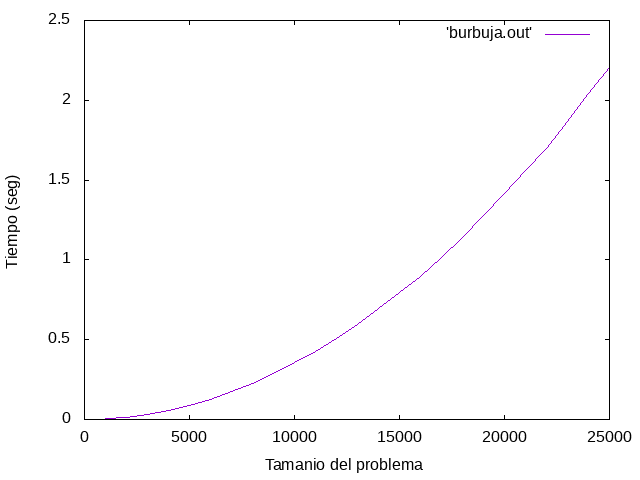
\includegraphics[scale=0.75]{empirica_burbuja.png}
\caption{Algoritmo burbuja}
\end{figure}

\begin{figure}[H]
\centering
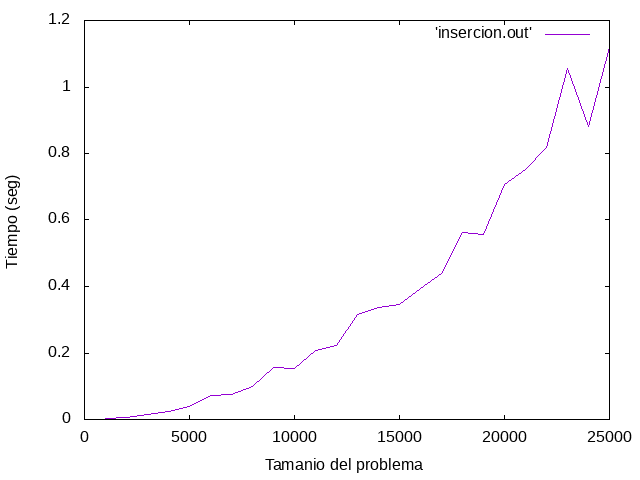
\includegraphics[scale=0.75]{empirica_insercion.png}
\caption{Algoritmo de inserción}
\end{figure}

\begin{figure}[H]
\centering
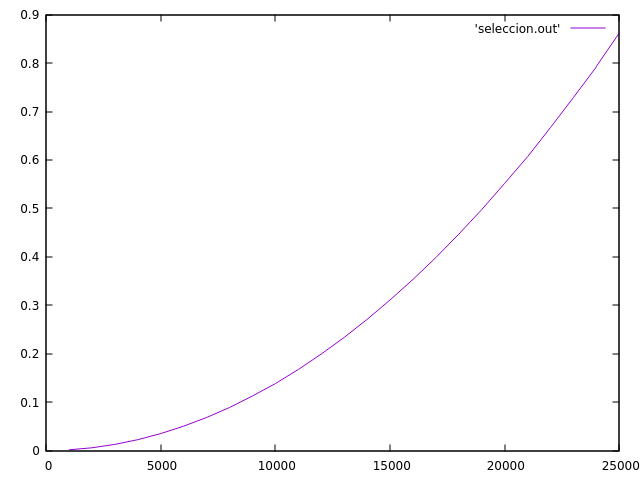
\includegraphics[scale=0.75]{empirica_seleccion.png}
\caption{Algoritmo de selección}
\end{figure}
\subsubsection{Algoritmo con eficiencia $O(n^3)$}
\begin{figure}[H]
\centering
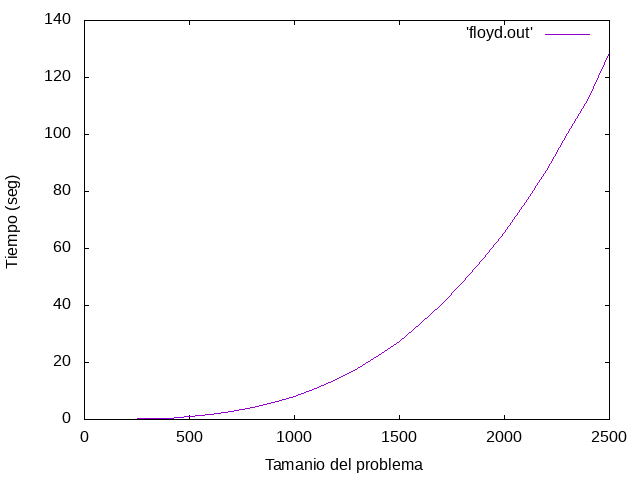
\includegraphics[scale=0.75]{empirica_floyd.png}
\caption{Algoritmo de Floyd}
\end{figure}

\subsubsection{Algoritmos con eficiencia $O(n \cdot log(n))$}

\begin{figure}[H]
\centering
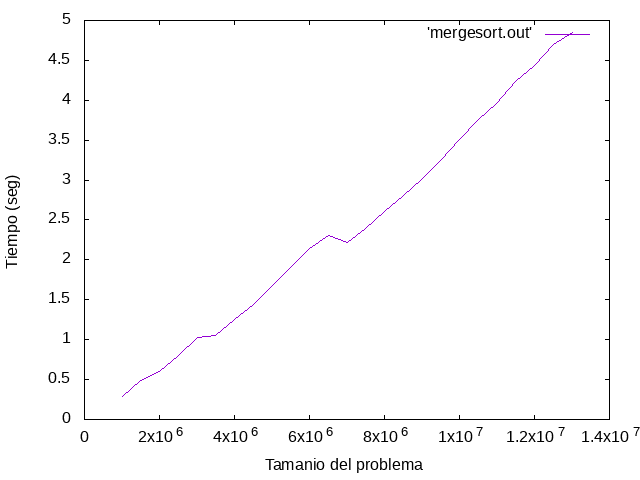
\includegraphics[scale=0.75]{empirica_mergesort.png}
\caption{Algoritmo mergesort}
\end{figure}

\begin{figure}[H]
\centering
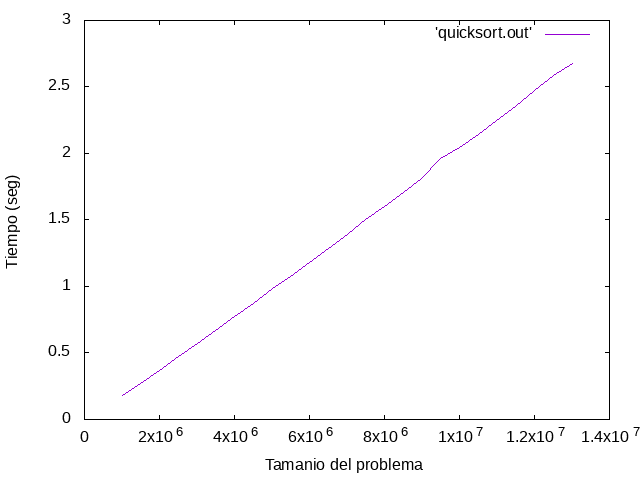
\includegraphics[scale=0.75]{empirica_quicksort.png}
\caption{Algoritmo quicksort}
\end{figure}

\begin{figure}[H]
\centering
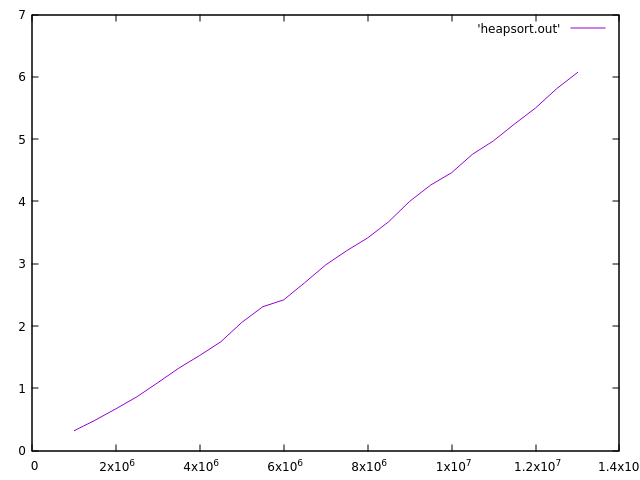
\includegraphics[scale=0.75]{empirica_heapsort.png}
\caption{Algoritmo heapsort}
\end{figure}

\subsubsection{Algoritmo con eficiencia $O(2^n)$}

\begin{figure}[H]
\centering
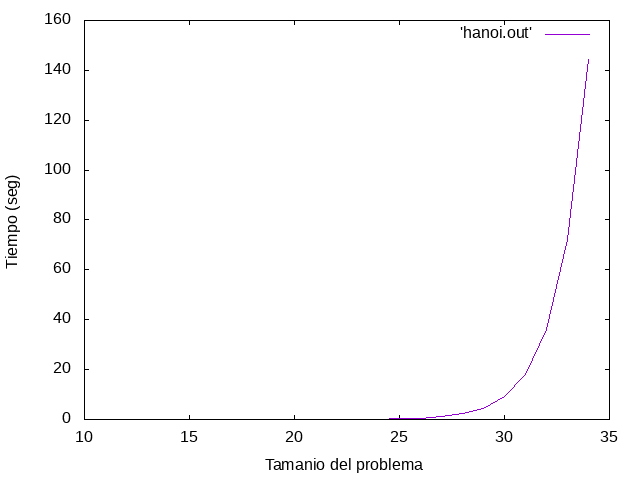
\includegraphics[scale=0.75]{empirica_hanoi.png}
\caption{Algoritmo Hanoi}
\end{figure}

\subsubsection{Comparación entre algoritmos de ordenación}
A simple vista solo podremos ver el trabajo de los algoritmos rápidos (\textit{heapsort}, \textit{mergesort} y \textit{quicksort}), ya que trabajan con tamaños de problema muy superiores al resto de algoritmos.

\begin{figure}[H]
\centering
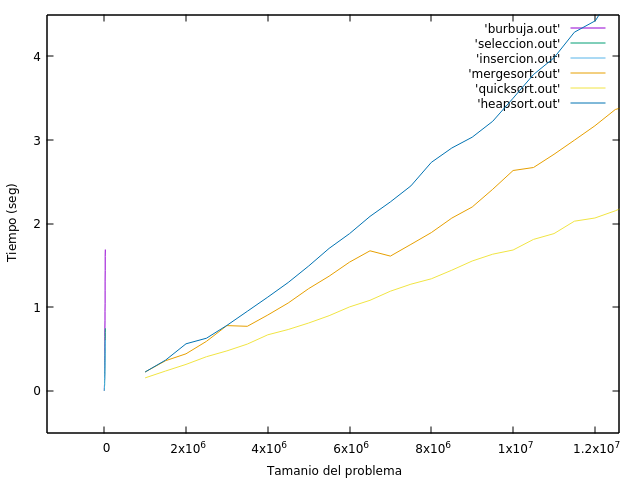
\includegraphics[scale=0.75]{empirica_ordenacion_comparacion.png}
\caption{Comparación de algoritmos de ordenación}
\end{figure}

Si hacemos zoom, podremos ver mejor la diferencia:

\begin{figure}[H]
\centering
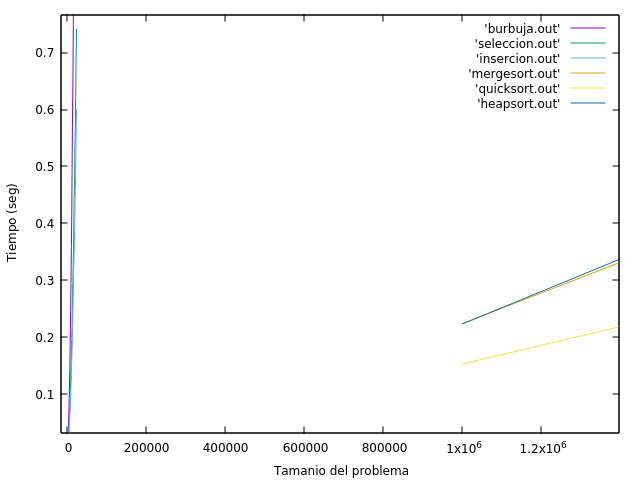
\includegraphics[scale=0.75]{empirica_ordenacion_comparacion_zoom.png}
\caption{Comparación de algoritmos de ordenación (zoom)}
\end{figure}
\subsection{Variación de la eficiencia empírica}
\label{sec:variacion}
\subsubsection{Entornos de ejecución}
\label{sec:entorno}
Todas las ejecuciones se realizarán en el \emph{PC 1}, excepto las que utilicemos para la comparación en el apartado de \textit{\nameref{sec:variacion}}.
\paragraph{PC 1}
\label{sec:pc1}
\begin{enumerate}
 \item CPU : AMD FX-8320 @3.50Ghz
  \begin{enumerate}
    \item Arquitectura : x86\_64
 	\item Caché
 	\begin{enumerate}
 		 \item Caché L1
 		\begin{enumerate}
 			 \item L1d : 16K
			 \item L1i : 64K 
 		 \end{enumerate}
		 \item Caché L2 : 2048K
 		 \item Caché L3 : 8192K
 	\end{enumerate}
 	 \item Frecuencia máxima (Overclock) : 4.20 Ghz
	 \item Núcleos físicos : 4
	 \item Núcleos lógicos : 8
	\end{enumerate}
	\item RAM
	\begin{enumerate}
	\item Capacidad : 16384 MB
	\item Frecuencia : 1600 Mhz
 	\item Tecnología : DDR3
	\end{enumerate}
\end{enumerate}
\paragraph{PC 2}
\label{sec:pc2}
\begin{enumerate}
\item CPU : Intel Core i7-6700HQ @2.60Ghz
\begin{enumerate}
	\item Arquitectura : x86\_64
	\item Caché
	\begin{enumerate}
		\item Caché L1
		\begin{enumerate}
			\item L1d : 32K
			\item L1i : 32K
		\end{enumerate}
		\item Caché L2 : 256K
		\item Caché L3 : 6144K
	\end{enumerate}
	\item Frecuencia máxima (HT) : 3.5 Ghz
	\item Núcleos físicos : 4
	\item Núcleos lógicos : 8
\end{enumerate}
\item RAM
\begin{enumerate}
	\item Capacidad : 8192 MB
 	\item Frecuencia : 2133 Mhz
 	\item Tecnología : DDR4
\end{enumerate}
\end{enumerate}

En esta sección demostraremos empíricamente el \emph{Principio de invarianza}.
\begin{ppio}[de Invarianza]
Dos implementaciones diferentes de un  mismo  algoritmo  no  difieren  en  eficiencia  más  que,  a  lo  sumo,  en  una constante multiplicativa.
\end{ppio}
Para ello, ejecutaremos los algoritmos en una arquitectura distinta, el \textit{\nameref{sec:pc2}}.
Comenzamos con una tabla donde podremos observar la constante en cuestión según el tiempo medio de ejecución de cada algoritmo:
\begin{table}[H]
\centering
\begin{tabular}{|c|c|c|c|}
\hline
\textbf{Algoritmo} & \textbf{Tiempo medio PC 1} & \textbf{Tiempo medio PC 2} & \textbf{Constante} \\
\hline
Burbuja & 0,366 & 0,251 & 1,456\\
\hline
Inserción & 0,172 & 0,100 & 1,715\\
\hline
\textit{Selección} & 0,144 & 0,124 & 1,159\\
\hline
\textit{Mergesort} & 1,948 & 1,422 & 1,371\\
\hline
\textit{Quicksort} & 1,144 & 0,965 & 1,186\\
\hline
\textit{Heapsort} & 2,314 & 1,821 & 1,271\\
\hline
Floyd & 8,636 & 5,348 & 1,615\\
\hline
Hanoi & 0,036 & 0,023 & 1,538\\
\hline
\end{tabular}
\caption{Comparación de tiempos entre ambos entornos de ejecución}
\end{table}
\subsubsection{Algoritmos con eficiencia $O(n^2)$}
\begin{figure}[H]
\centering
\begin{subfigure}[b]{0.45\textwidth}
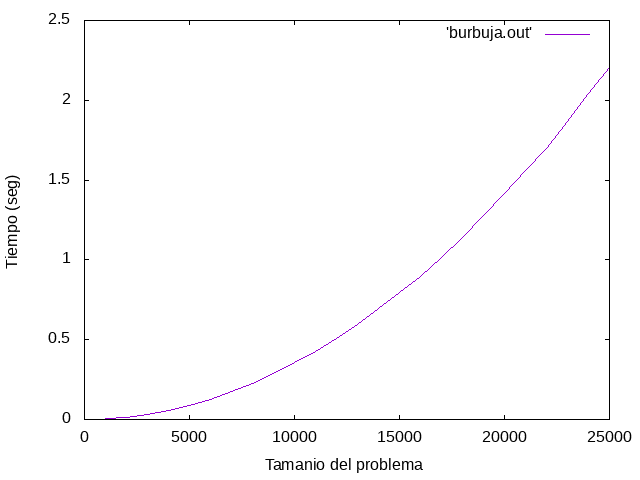
\includegraphics[scale=0.45]{empirica_burbuja.png}
\caption{\nameref{sec:pc1}}
\end{subfigure}
\quad
\begin{subfigure}[b]{0.45\textwidth}
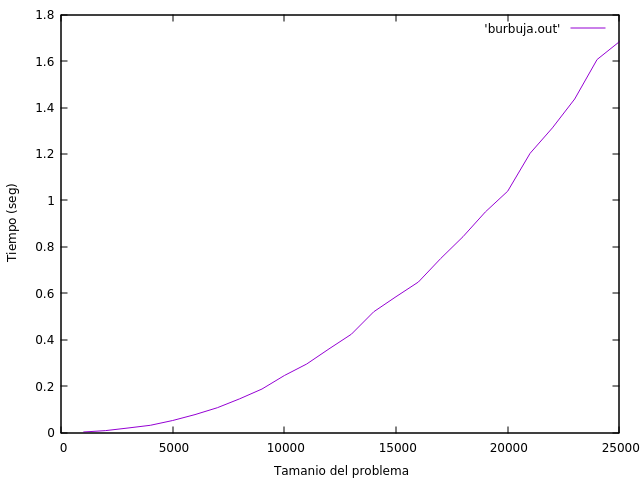
\includegraphics[scale=0.45]{empirica_burbuja_2.png}
\caption{\nameref{sec:pc2}}
\end{subfigure}
\newline
\newline
\begin{tabular}{|c|c|c|}
\hline
\textbf{Tamaño} & \textbf{Tiempo PC 1} & \textbf{Tiempo PC 2} \\
\hline
1000 & 0.00347 & 0.002096 \\
\hline
2000 & 0.014092 & 0.008327 \\
\hline
3000 & 0.031775 & 0.019441 \\
\hline
4000 & 0.056423 & 0.031218 \\
\hline
5000 & 0.088117 & 0.051639\\
\hline
6000 & 0.127298 & 0.07696\\
\hline
7000 & 0.174768 & 0.106872\\
\hline
8000 & 0.227671 & 0.145037\\
\hline
9000 & 0.287853 & 0.187409\\
\hline
10000 & 0.355994 & 0.245409\\
\hline
11000 & 0.427654 & 0.295032\\
\hline
12000 & 0.509095 & 0.359974\\
\hline
13000 & 0.597057 & 0.423534\\
\hline
14000 & 0.693367 & 0.520076\\
\hline
15000 & 0.796559 & 0.584748\\
\hline
16000 & 0.898766 & 0.648439\\
\hline
17000 & 1.01542 & 0.749665\\
\hline
18000 & 1.14065 & 0.843255\\
\hline
19000 & 1.27787 & 0.950054\\
\hline
20000 & 1.41778 & 1.03928\\
\hline
21000 & 1.56071 & 1.20255\\
\hline
22000 & 1.70092 & 1.31179\\
\hline
23000 & 1.86982 & 1.4365\\
\hline
24000 & 2.04169 & 1.60665\\
\hline
25000 & 2.20676 & 1.68318 \\
\hline
\end{tabular}
\caption{Algoritmo burbuja}
\end{figure}

\begin{figure}[H]
\centering
\begin{subfigure}[b]{0.45\textwidth}
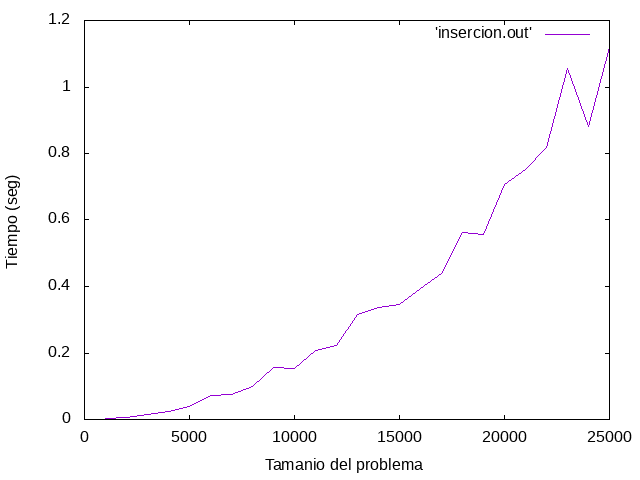
\includegraphics[scale=0.45]{empirica_insercion.png}
\caption{\nameref{sec:pc1}}
\end{subfigure}
\quad
\begin{subfigure}[b]{0.45\textwidth}
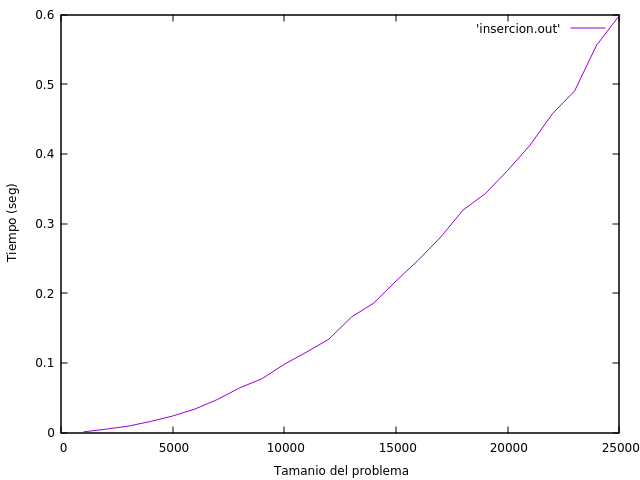
\includegraphics[scale=0.45]{empirica_insercion_2.png}
\caption{\nameref{sec:pc2}}
\end{subfigure}
\newline
\newline
\begin{tabular}{|c|c|c|}
\hline
\textbf{Tamaño} & \textbf{Tiempo PC 1} & \textbf{Tiempo PC 2} \\
\hline
1000  & 0,001566 & 0,000911 \\
\hline
2000  & 0,006863 & 0,004746\\
\hline
3000  & 0,013775 & 0,009101\\
\hline
4000  & 0,024662 & 0,015753\\
\hline
5000  & 0,038397 & 0,023742\\
\hline
6000  & 0,073059 & 0,033688\\
\hline
7000  & 0,075398 & 0,047426\\
\hline
8000  & 0,097854 & 0,064051\\
\hline
9000  & 0,157555 & 0,077217\\
\hline
10000 & 0,15269  & 0,098011\\
\hline
11000 & 0,207507 &  0,115522\\
\hline
12000 & 0,221672 &  0,134134\\
\hline
13000 & 0,315095 &  0,165736\\
\hline
14000 & 0,337785 & 0,185779\\
\hline
15000 & 0,345627 & 0,217502\\
\hline
16000 & 0,393965 & 0,247678\\
\hline
17000 & 0,438195 & 0,280534\\
\hline
18000 & 0,563423 & 0,319248\\
\hline
19000 & 0,555218 & 0,343008\\
\hline
20000 & 0,707812 & 0,376268\\
\hline
21000 & 0,752603 & 0,41259\\
\hline
22000 & 0,817934 & 0,457614\\
\hline
23000 & 1,05414  & 0,490588\\
\hline
24000 & 0,881149 & 0,557605\\
\hline
25000 & 1,11894  & 0,599629\\
\hline
\end{tabular}
\caption{Algoritmo de inserción}
\end{figure}

\begin{figure}[H]
\centering
\begin{subfigure}[b]{0.45\textwidth}
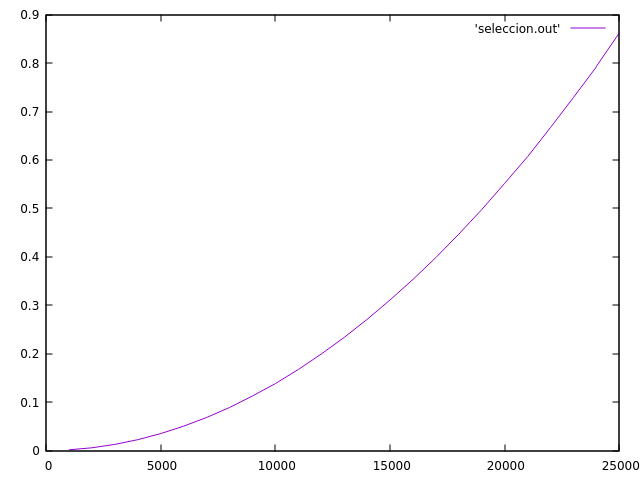
\includegraphics[scale=0.45]{empirica_seleccion.png}
\caption{\nameref{sec:pc1}}
\end{subfigure}
\quad
\begin{subfigure}[b]{0.45\textwidth}
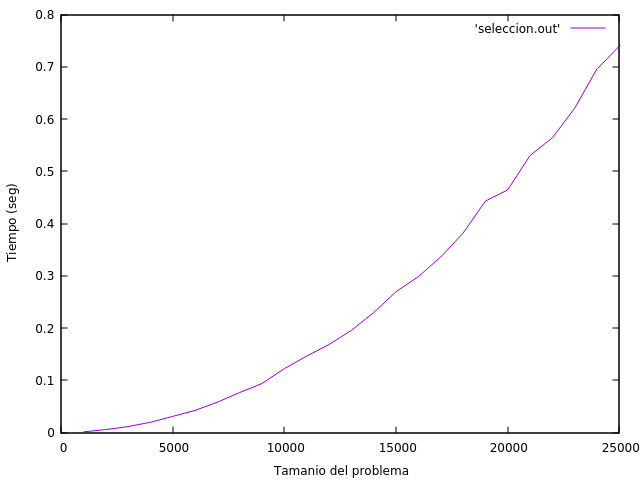
\includegraphics[scale=0.45]{empirica_seleccion_2.png}
\caption{\nameref{sec:pc2}}
\end{subfigure}
\newline
\newline
\begin{tabular}{|c|c|c|}
\hline
\textbf{Tamaño} & \textbf{Tiempo PC 1} & \textbf{Tiempo PC 2} \\
\hline
1000 & 0,001469 & 0,001203 \\
\hline
2000 & 0,005661 & 0,005539\\
\hline
3000 & 0,012639 & 0,011269\\
\hline
4000 & 0,022373 & 0,019565\\
\hline
5000 & 0,0348 & 0,030867\\
\hline
6000 & 0,050395 & 0,042368\\
\hline
7000 & 0,06795 & 0,057941\\
\hline
8000 & 0,088633 & 0,076493\\
\hline
9000 & 0,112056 & 0,093877\\
\hline
10000 & 0,138403 & 0,122324\\
\hline
11000 & 0,167213 & 0,146299\\
\hline
12000 & 0,198844 & 0,168477\\
\hline
13000 & 0,233619 & 0,195566\\
\hline
14000 & 0,270472 & 0,229449\\
\hline
15000 & 0,310389 & 0,269606\\
\hline
16000 & 0,353077 & 0,298446\\
\hline
17000 & 0,398466 & 0,336024\\
\hline
18000 & 0,447165 & 0,38157\\
\hline
19000 & 0,497554 & 0,442948\\
\hline
20000 & 0,551222 & 0,464486\\
\hline
21000 & 0,607534 & 0,530445\\
\hline
22000 & 0,667603 & 0,564229\\
\hline
23000 & 0,728555 & 0,620878\\
\hline
24000 & 0,793231 & 0,696617\\
\hline
25000 & 0,8607 & 0,740901\\
\hline
\end{tabular}
\caption{Algoritmo de selección}
\end{figure}
\subsubsection{Algoritmos con eficiencia $O(n^3)$}

\begin{figure}[H]
\centering
\begin{subfigure}[b]{0.45\textwidth}
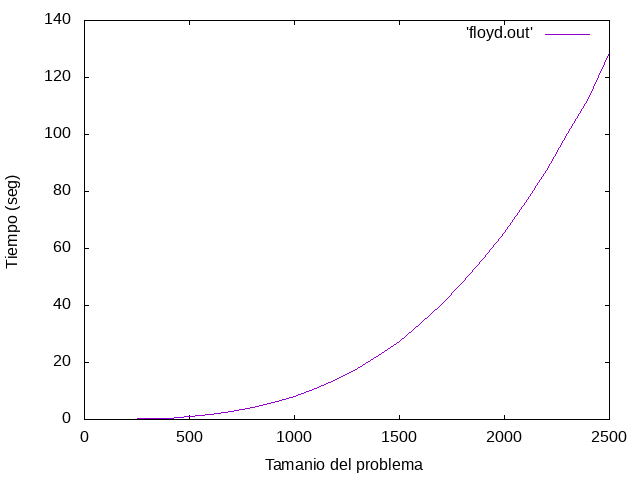
\includegraphics[scale=0.45]{empirica_floyd.png}
\caption{\nameref{sec:pc1}}
\end{subfigure}
\quad
\begin{subfigure}[b]{0.45\textwidth}
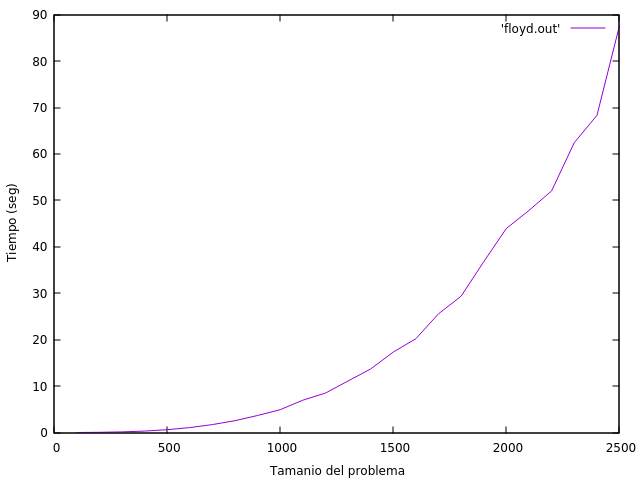
\includegraphics[scale=0.45]{empirica_floyd_2.png}
\caption{\nameref{sec:pc2}}
\end{subfigure}
\newline
\newline
\begin{tabular}{|c|c|c|}
\hline
\textbf{Tamaño} & \textbf{Tiempo PC 1} & \textbf{Tiempo PC 2} \\
\hline
100 & 0,008394 & 0,005113\\
\hline
200 & 0,066017 & 0,041535\\
\hline
300 & 0,220825 & 0,138818\\
\hline
400 & 0,521858 & 0,311018\\
\hline
500 & 1,01887 & 0,602487\\
\hline
600 & 1,75665 & 1,05512\\
\hline
700 & 2,80066 & 1,70498\\
\hline
800 & 4,17319 & 2,5442\\
\hline
900 & 5,95085 & 3,65579\\
\hline
1000 & 8,15234 & 4,91424\\
\hline
1100 & 10,8509 & 6,95897\\
\hline
1200 & 14,0868 & 8,47521\\
\hline
1300 & 17,9348 & 11,0851\\
\hline
1400 & 22,3625 & 13,6728\\
\hline
1500 & 27,532 & 17,3226\\
\hline
1600 & 33,5096 & 20,2078\\
\hline
1700 & 40,3014 & 25,5719\\
\hline
1800 & 47,9103 & 29,3598\\
\hline
1900 & 56,4474 & 36,773\\
\hline
2000 & 65,7778 & 43,9358\\
\hline
2100 & 76,1326 & 47,8074\\
\hline
2200 & 87,528 & 52,0403\\
\hline
2300 & 100,508 & 62,3899\\
\hline
2400 & 112,763 & 68,2729\\
\hline
2500 & 128,779 & 87,6574\\
\hline
\end{tabular}
\caption{Algoritmo de Floyd}
\end{figure}

\subsubsection{Algoritmos con eficiencia $O(n \cdot log(n))$}

\begin{figure}[H]
\centering
\begin{subfigure}[b]{0.45\textwidth}
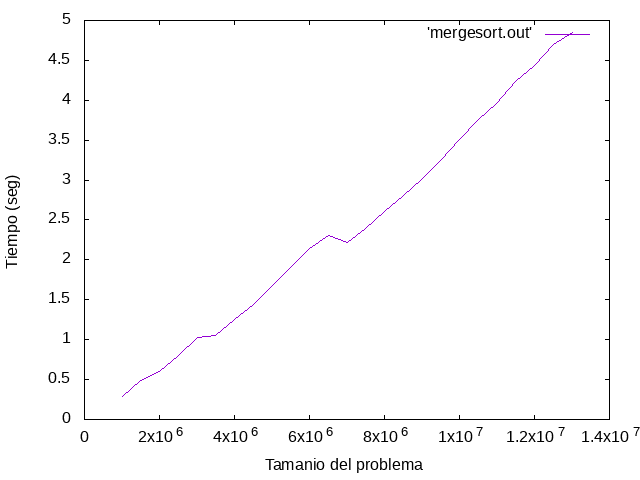
\includegraphics[scale=0.45]{empirica_mergesort.png}
\caption{\nameref{sec:pc1}}
\end{subfigure}
\quad
\begin{subfigure}[b]{0.45\textwidth}
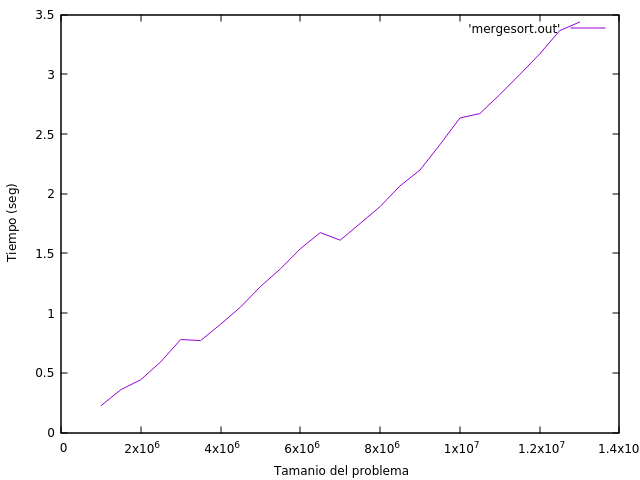
\includegraphics[scale=0.45]{empirica_mergesort_2.png}
\caption{\nameref{sec:pc2}}
\end{subfigure}
\newline
\newline
\begin{tabular}{|c|c|c|}
\hline
\textbf{Tamaño} & \textbf{Tiempo PC 1} & \textbf{Tiempo PC 2} \\
\hline
1000000 & 0,284222d & 0,224028 \\
\hline
1500000 & 0,493673d & 0,358624 \\
\hline
2000000 & 0,597351d & 0,442203 \\
\hline
2500000 & 0,796508d & 0,591356 \\
\hline
3000000 & 1,03026d & 0,778666 \\
\hline
3500000 & 1,05322d & 0,770087 \\
\hline
4000000 & 1,25594d & 0,905945 \\
\hline
4500000 & 1,44694d & 1,0499 \\
\hline
5000000 & 1,6732d & 1,22218 \\
\hline
5500000 & 1,90594d & 1,37029 \\
\hline
6000000 & 2,14261d & 1,53875 \\
\hline
6500000 & 2,30352d & 1,67414 \\
\hline
7000000 & 2,21224d & 1,61097 \\
\hline
7500000 & 2,39566d & 1,75056 \\
\hline
8000000 & 2,60288d & 1,89201 \\
\hline
8500000 & 2,81016d & 2,06572 \\
\hline
9000000 & 3,00176d & 2,19856 \\
\hline
9500000 & 3,24843d & 2,41008 \\
\hline
10000000 & 3,50923d & 2,63424 \\
\hline
10500000 & 3,76182d & 2,67053 \\
\hline
11000000 & 3,95387d & 2,82914 \\
\hline
11500000 & 4,23099d & 2,99723 \\
\hline
12000000 & 4,43627d & 3,16933 \\
\hline
12500000 & 4,7013d & 3,36511 \\
\hline
13000000 & 4,84492d & 3,43713 \\
\hline
\end{tabular}
\caption{Algoritmo mergesort}
\end{figure}

\begin{figure}[H]
\centering
\begin{subfigure}[b]{0.45\textwidth}
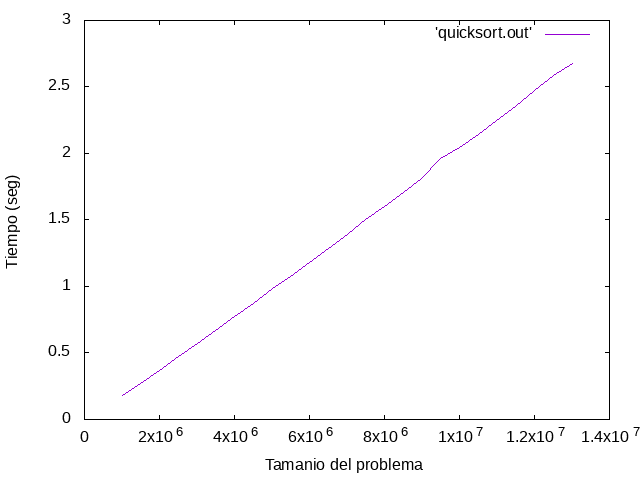
\includegraphics[scale=0.45]{empirica_quicksort.png}
\caption{\nameref{sec:pc1}}
\end{subfigure}
\quad
\begin{subfigure}[b]{0.45\textwidth}
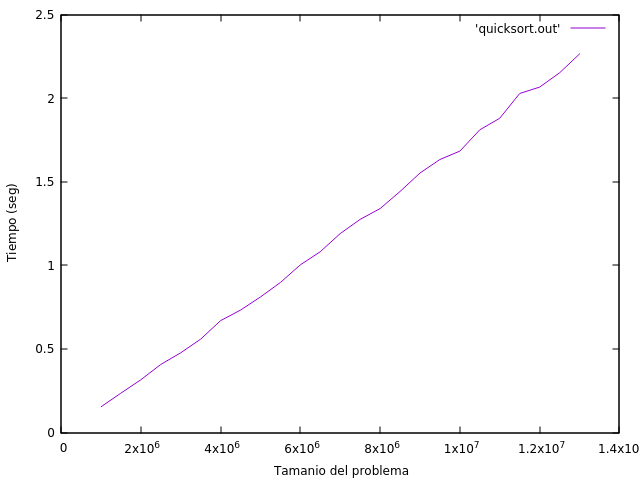
\includegraphics[scale=0.45]{empirica_quicksort_2.png}
\caption{\nameref{sec:pc2}}
\end{subfigure}
\newline
\newline
\begin{tabular}{|c|c|c|}
\hline
\textbf{Tamaño} & \textbf{Tiempo PC 1} & \textbf{Tiempo PC 2} \\
\hline
1000000 & 0,179104 & 0,153138 \\
\hline
1500000 & 0,272898 & 0,235349 \\
\hline
2000000 & 0,372015 & 0,315383 \\
\hline
2500000 & 0,474955 & 0,40695 \\
\hline
3000000 & 0,57355 & 0,476882 \\
\hline
3500000 & 0,671565 & 0,557988 \\
\hline
4000000 & 0,772 & 0,668801 \\
\hline
4500000 & 0,874961 & 0,732228 \\
\hline
5000000 & 0,984274 & 0,810474 \\
\hline
5500000 & 1,07864 & 0,897322 \\
\hline
6000000 & 1,18198 & 1,00255 \\
\hline
6500000 & 1,2892 & 1,08152 \\
\hline
7000000 & 1,39126 & 1,19 \\
\hline
7500000 & 1,50179 & 1,2749 \\
\hline
8000000 & 1,60031 & 1,33935 \\
\hline
8500000 & 1,70584 & 1,44181 \\
\hline
9000000 & 1,81074 & 1,55247 \\
\hline
9500000 & 1,95951 & 1,63309 \\
\hline
10000000 & 2,04412 & 1,68327 \\
\hline
10500000 & 2,14102 & 1,81085 \\
\hline
11000000 & 2,25131 & 1,87967 \\
\hline
11500000 & 2,35475 & 2,02783 \\
\hline
12000000 & 2,47356 & 2,06599 \\
\hline
12500000 & 2,58437 & 2,15211 \\
\hline
13000000 & 2,67631 & 2,26403 \\
\hline
\end{tabular}
\caption{Algoritmo quicksort}
\end{figure}

\begin{figure}[H]
\centering
\begin{subfigure}[b]{0.45\textwidth}
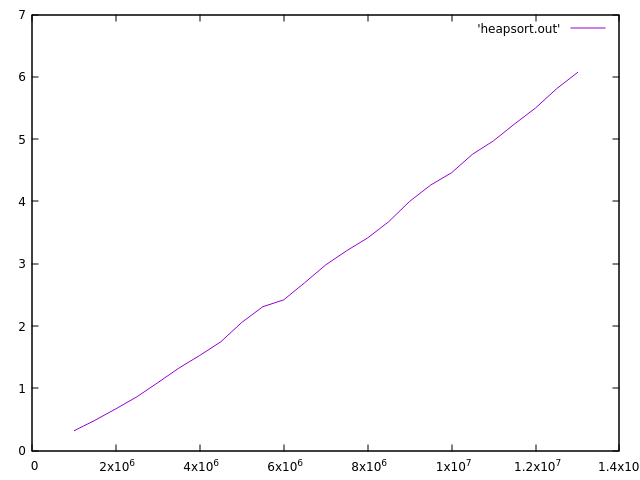
\includegraphics[scale=0.45]{empirica_heapsort.png}
\caption{\nameref{sec:pc1}}
\end{subfigure}
\quad
\begin{subfigure}[b]{0.45\textwidth}
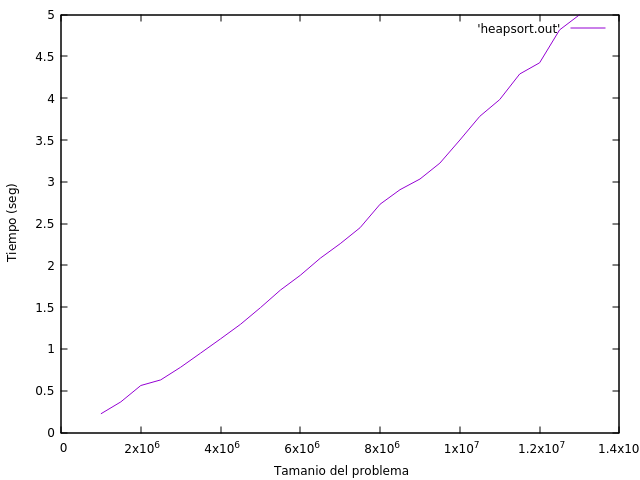
\includegraphics[scale=0.45]{empirica_heapsort_2.png}
\caption{\nameref{sec:pc2}}
\end{subfigure}
\newline
\newline
\begin{tabular}{|c|c|c|}
\hline
\textbf{Tamaño} & \textbf{Tiempo PC 1} & \textbf{Tiempo PC 2} \\
\hline
1000000 & 0,313202d & 0,223356 \\
\hline
1500000 & 0,482248d & 0,366004\\
\hline
2000000 & 0,664047d & 0,561854\\
\hline
2500000 & 0,855399d & 0,628741\\
\hline
300000 & 1,05215d & 0,781531\\
\hline
350000 & 1,27027d & 0,949929\\
\hline
400000 & 1,47906d & 1,1197\\
\hline
450000 & 1,69867d & 1,29438\\
\hline
500000 & 1,91449d & 1,49264\\
\hline
550000 & 2,15878d & 1,70317\\
\hline
600000 & 2,38723d & 1,88031\\
\hline
650000 & 2,61876d & 2,08545\\
\hline
700000 & 2,86654d & 2,25945\\
\hline
750000 & 3,12018d & 2,45073\\
\hline
800000 & 3,39958d & 2,73144\\
\hline
850000 & 3,63556d & 2,90442\\
\hline
900000 & 3,90373d & 3,03281\\
\hline
950000 & 4,14154d & 3,22381\\
\hline
1000000 & 4,39101d & 3,50009\\
\hline
1050000 & 4,64831d & 3,78361\\
\hline
1100000 & 4,90958d & 3,98295\\
\hline
1150000 & 5,17252d & 4,28962\\
\hline
1200000 & 5,45655d & 4,42294\\
\hline
1250000 & 5,72861d & 4,81687\\
\hline
1300000 & 5,99094d & 4,99741\\
\hline
\end{tabular}
\caption{Algoritmo heapsort}
\end{figure}

\subsubsection{Algoritmo con eficiencia $O(2^n)$}

\begin{figure}[H]
\centering
\begin{subfigure}[b]{0.45\textwidth}
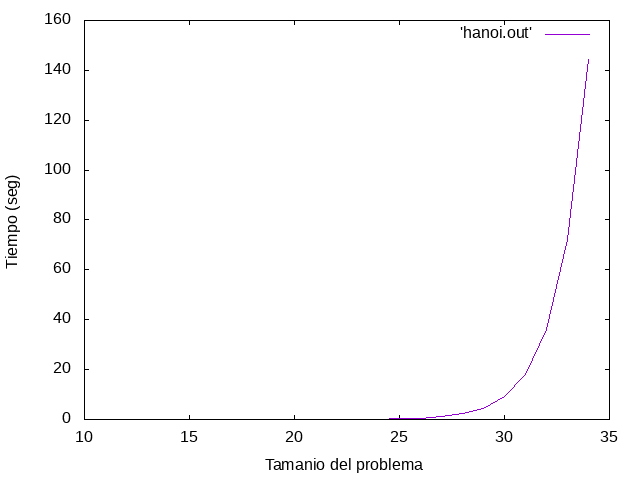
\includegraphics[scale=0.45]{empirica_hanoi.png}
\caption{\nameref{sec:pc1}}
\end{subfigure}
\quad
\begin{subfigure}[b]{0.45\textwidth}
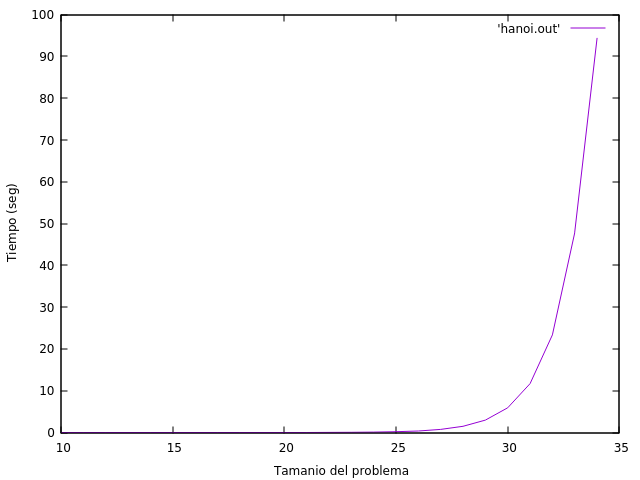
\includegraphics[scale=0.45]{empirica_hanoi_2.png}
\caption{\nameref{sec:pc2}}
\end{subfigure}
\newline
\newline
\begin{tabular}{|c|c|c|}
\hline
\textbf{Tamaño} & \textbf{Tiempo PC 1} & \textbf{Tiempo PC 2} \\
\hline
10 & 1,00E-05 & 7,00E-06\\
\hline
11 & 1,80E-05 & 1,20E-05\\
\hline
12 & 3,60E-05 & 2,50E-05\\
\hline
13 & 7,30E-05 & 4,50E-05\\
\hline
14 & 0,000145 & 8,90E-05\\
\hline
15 & 0,000288 & 0,000176\\
\hline
16 & 0,000587 & 0,000352\\
\hline
17 & 0,001131 & 0,000853\\
\hline
18 & 0,002277 & 0,001464\\
\hline
19 & 0,004491 & 0,002866\\
\hline
20 & 0,008952 & 0,00571\\
\hline
21 & 0,017783 & 0,011502\\
\hline
22 & 0,035699 & 0,022844\\
\hline
23 & 0,071711 & 0,045985\\
\hline
24 & 0,142219 & 0,092678\\
\hline
25 & 0,284257 & 0,181169\\
\hline
26 & 0,564716 & 0,364107\\
\hline
27 & 1,13561 & 0,741404\\
\hline
28 & 2,25519 & 1,49178\\
\hline
29 & 4,51148 & 2,96788\\
\hline
30 & 9,03096 & 5,9088\\
\hline
31 & 18,0955 & 11,7069\\
\hline
32 & 36,0193 & 23,3482\\
\hline
33 & 72,2035 & 47,761\\
\hline
34 & 144,474 & 94,3148\\
\hline
\end{tabular}
\caption{Algoritmo de Hanoi}
\end{figure}
\newpage
\section{Cálculo de la eficiencia híbrida}
Para realizar este cálculo, realizamos una regresión de la expresión de eficiencia teórica con respecto a los datos empíricos obtenidos.\\
Si nuestros datos son correctos, el porcentaje de error será muy bajo.
\begin{table}[H]
\centering
\begin{tabular}{|c|c|c|}
\hline
\textbf{Algoritmo} & \textbf{Orden de eficiencia} & \textbf{Porcentaje de error} \\
\hline
Burbuja &  & 2.253e-12 (0.06377\%)\\
Selección & $n^2$ & 3.047e-13 (0.02211\%)\\
Inserción & & 3.085e-11 (1.805\%) \\
\hline
Heapsort &  & 2.071e-10 (0.7626\%) \\
Mergesort & $n \cdot log(n)$ & 1.893e-10 (0.8614\%) \\
Quicksort & & 1.407e-11 (0.1113\%) \\
\hline
Hanoi & $2^n$ & 1.095e-12 (0.01302\%) \\
\hline
Floyd & $n^3$ & 7.291e-12 (0.08874\%) \\
\hline
{\color{red}Ajuste erróneo} & {\color{red}$2^n$ a $n^2$} & {\color{red}0.00868(26.86\%)}\\
\hline
\end{tabular}
\caption{Bondad de los ajustes}
\end{table}

\subsection{Algoritmos con eficiencia $O(n^2)$}

\begin{figure}[H]
\centering
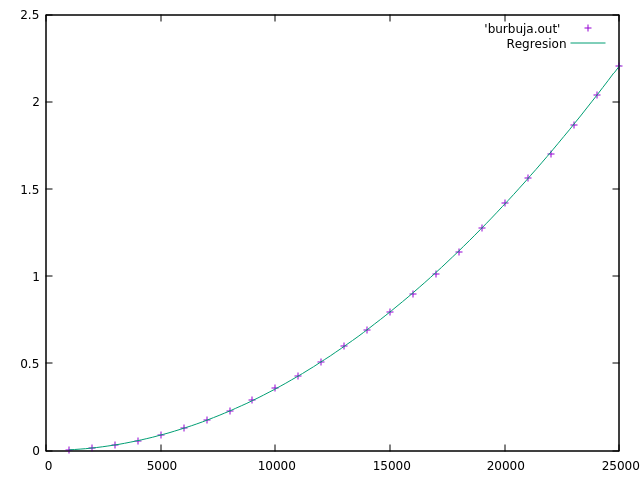
\includegraphics[scale=0.75]{hibrida_burbuja.png}
\caption{Algoritmo burbuja}
\end{figure}

\begin{figure}[H]
\centering
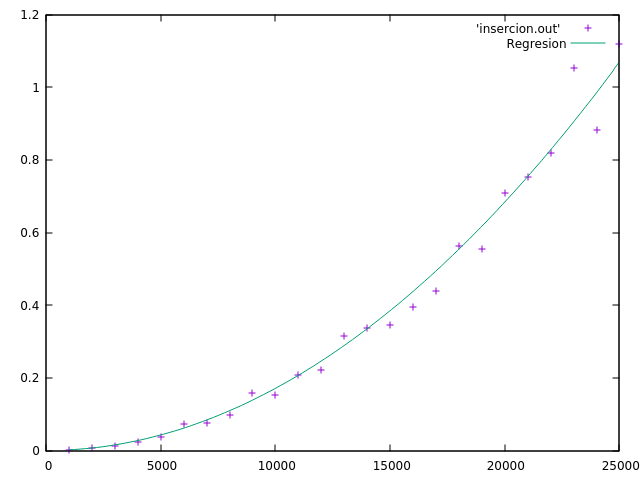
\includegraphics[scale=0.75]{hibrida_insercion.png}
\caption{Algoritmo de inserción}
\end{figure}

\begin{figure}[H]
\centering
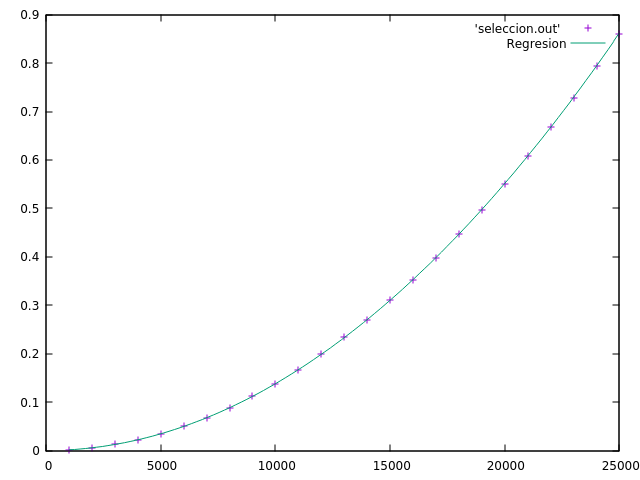
\includegraphics[scale=0.75]{hibrida_seleccion.png}
\caption{Algoritmo de selección}
\end{figure}

\subsection{Algoritmo con eficiencia $O(n^3)$}

\begin{figure}[H]
\centering
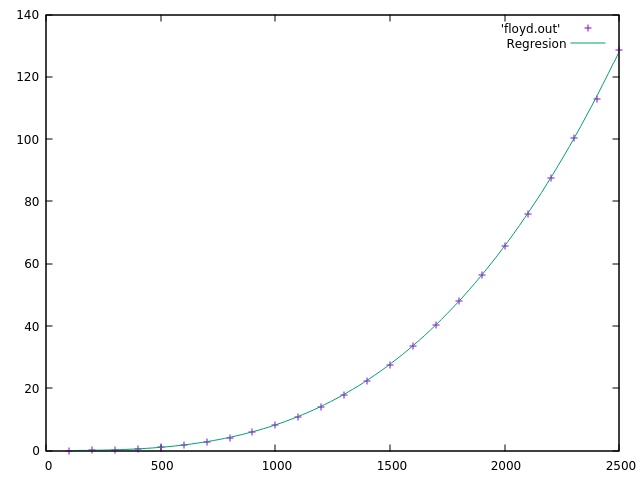
\includegraphics[scale=0.75]{hibrida_floyd.png}
\caption{Algoritmo de Floyd}
\end{figure}

\subsection{Algoritmos con eficiencia $O(n \cdot log(n))$}

\begin{figure}[H]
\centering
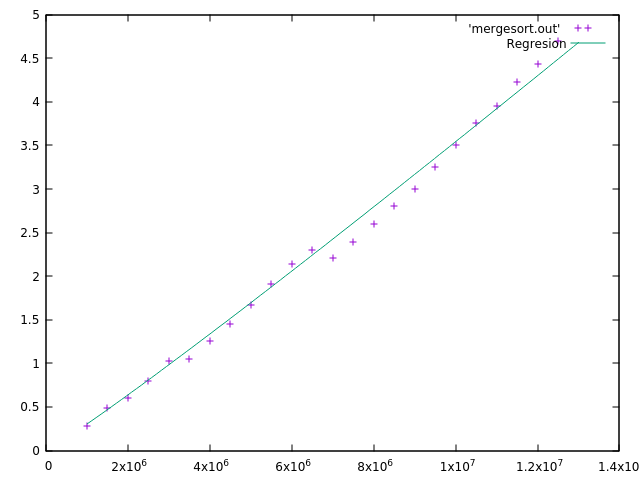
\includegraphics[scale=0.75]{hibrida_mergesort.png}
\caption{Algoritmo mergesort}
\end{figure}

\begin{figure}[H]
\centering
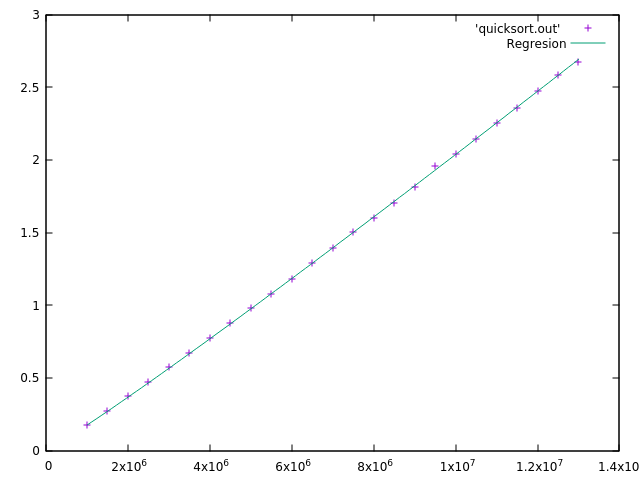
\includegraphics[scale=0.75]{hibrida_quicksort.png}
\caption{Algoritmo quicksort}
\end{figure}

\begin{figure}[H]
\centering
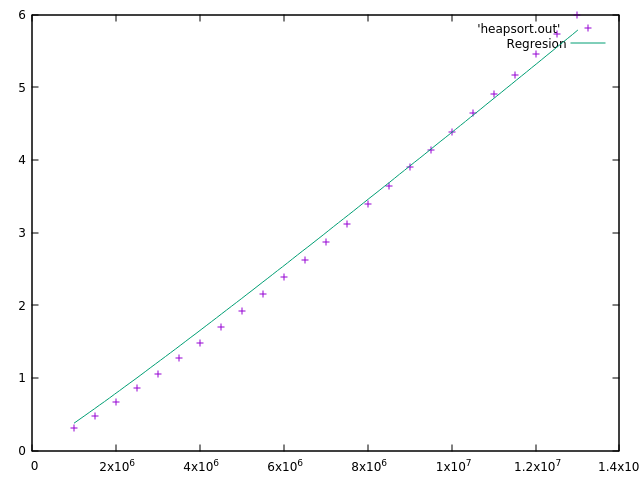
\includegraphics[scale=0.75]{hibrida_heapsort.png}
\caption{Algoritmo heapsort}
\end{figure}

\subsection{Algoritmo con eficiencia $O(2^n)$}

\begin{figure}[H]
\centering
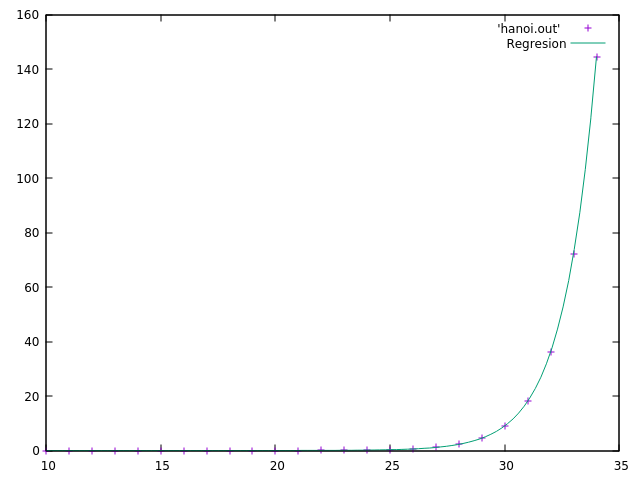
\includegraphics[scale=0.75]{hibrida_hanoi.png}
\caption{Algoritmo Hanoi}
\end{figure}

\newpage

\subsection{Ajuste erróneo}
Aquí ajustamos los datos del Algoritmo de Hanoi ($O(2^n)$) a una eficiencia teórica cuadrática ($O(n^2)$). Vemos que además de obtener muchísimo error, la gráfica no es consistente.

\begin{figure}[H]
\centering
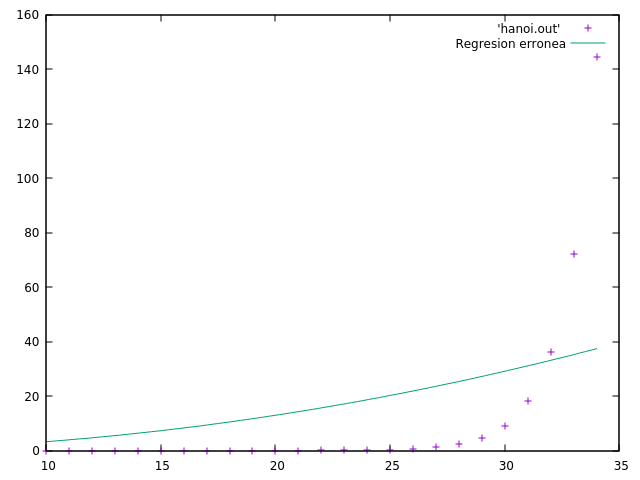
\includegraphics[scale=0.75]{ajuste_erroneo.png}
\caption{Regresión errónea}
\end{figure}
\newpage
\section{Anexo: Código fuente utilizado}

Los algoritmos empleados para realizar la práctica han sido descargados de la plataforma \textit{decsai.ugr.es}.
\subsection{Hanoi}
\begin{multicols}{2}
\begin{tcblisting}{
  enhanced,
  listing only,
  minted options={
    baselinestretch=1.0,
    %bgcolor=lightgray,
    fontsize=\footnotesize,
    linenos,
    breaklines,
  },
  minted language=c++,
  boxrule=0pt,
  boxsep=0pt,
  frame hidden,
  breakable=unlimited,
}  
#include <iostream>
using namespace std;
#include <ctime>
#include <cstdlib>

/**
   @brief Resuelve el problema de las Torres de Hanoi
   @param M: número de discos. M > 1.
   @param i: número de columna en que están los discos.
             i es un valor de {1, 2, 3}. i != j.
   @param j: número de columna a que se llevan los discos.
             j es un valor de {1, 2, 3}. j != i.

   Esta función imprime en la salida estándar la secuencia de 
   movimientos necesarios para desplazar los M discos de la
   columna i a la j, observando la restricción de que ningún
   disco se puede situar sobre otro de tamaño menor. Utiliza
   una única columna auxiliar.
*/
void hanoi (int M, int i, int j);

void hanoi (int M, int i, int j)
{
  if (M > 0)
    {
      hanoi(M-1, i, 6-i-j);
      cout << i << " -> " << j << endl;
      hanoi (M-1, 6-i-j, j);
  }
}

int main(int argc, char * argv[])
{
  
    if (argc != 2)
    {
      cerr << "Formato " << argv[0] << " <num_discos>" << endl;
      return -1;
    }

  int M = atoi(argv[1]);

  clock_t tantes;    // Valor del reloj antes de la ejecución
  clock_t tdespues;  // Valor del reloj después de la ejecución
  tantes = clock();
  hanoi(M, 1, 2);
  tdespues = clock();
  cout << M << 
  ((double)(tdespues-tantes))
  /CLOCKS_PER_SEC << endl; 
  return 0;
}
\end{tcblisting}
\end{multicols}
\newpage

\subsection{Floyd}
\begin{multicols}{2}
\begin{tcblisting}
{
  enhanced,
  listing only,
  minted options={
    baselinestretch=1.0,
    fontsize=\footnotesize,
    linenos,
    breaklines,
  },
  minted language=c++,
  boxrule=0pt,
  boxsep=0pt,
  frame hidden,
  breakable=unlimited,
}
  
#include <iostream>
using namespace std;
#include <ctime>
#include <cstdlib>
#include <climits>
#include <cassert>
#include <cmath>

static int const MAX_LONG  = 10;
            
/**
   @brief Reserva espacio en memoria dinámica para una matriz cuadrada.
   
   @param dim: dimensión de la matriz. dim > 0.

   @returns puntero a la zona de memoria reservada.
*/
int ** ReservaMatriz(int dim);

/**
   @brief Libera el espacio asignado a una matriz cuadrada.
   
   @param M: puntero a la zona de memoria reservada. Es MODIFICADO.
   @param dim: dimensión de la matriz. dim > 0.

   Liberar la zona memoria asignada a M y lo pone a NULL.
*/
void LiberaMatriz(int ** & M, int dim);

/**
   @brief Rellena una matriz cuadrada con valores aleaotorias.
   
   @param M: puntero a la zona de memoria reservada. Es MODIFICADO.
   @param dim: dimensión de la matriz. dim > 0.

   Asigna un valor aleatorio entero de [0, MAX_LONG - 1] a cada
   elemento de la matriz M, salvo los de la diagonal principal
   que quedan a 0..
*/
void RellenaMatriz(int **M, int dim);

/**
   @brief Cálculo de caminos mínimos.
   
   @param M: Matriz de longitudes de los caminos. Es MODIFICADO.
   @param dim: dimensión de la matriz. dim > 0.

   Calcula la longitud del camino mínimo entre cada par de nodos (i,j),
   que se almacena en M[i][j].
*/
void Floyd(int **M, int dim);


/**
   Implementación de las funciones
**/

int ** ReservaMatriz(int dim)
{
  int **M;
  if (dim  <= 0)
    {
      cerr<< "\n ERROR: Dimension de la matriz debe ser mayor que 0" << endl;
      exit(1);
    }
  M = new int * [dim];
  if (M == NULL)
    {
      cerr << "\n ERROR: No puedo reservar memoria para un matriz de "
 &    << dim << " x " << dim << "elementos" << endl;
      exit(1);
    }
  for (int i = 0; i < dim; i++)
    {
      M[i]= new int [dim];
      if (M[i] == NULL)
 & {
 &   cerr << "ERROR: No puedo reservar memoria para un matriz de "
 &        << dim << " x " << dim << endl;
 &   for (int j = 0; j < i; j++)
 &     delete [] M[i];
 &   delete [] M;
 &   exit(1);
 & } 
    }
  return M;
} & 

void LiberaMatriz(int ** & M, int dim)
{
  for (int i = 0; i < dim; i++)
    delete [] M[i];
  delete [] M;
  M = NULL;
} &  & 


void RellenaMatriz(int **M, int dim)
{
  for (int i = 0; i < dim; i++)
    for (int j = 0; j < dim; j++)
      if (i != j)
 & M[i][j]= (rand() \% MAX_LONG);
} &  &  & 
 & 
void Floyd(int **M, int dim)
{
 & for (int k = 0; k < dim; k++)
 &   for (int i = 0; i < dim;i++)
 &     for (int j = 0; j < dim;j++)
 &       {
 &  & int sum = M[i][k] + M[k][j];     & 
 &      & M[i][j] = (M[i][j] > sum) ? sum : M[i][j];
 &       }
} &       & 

int main (int argc, char **argv)
{
//  clock_t tantes;   
//  clock_t tdespues;
    int dim;          

  //Lectura de los parametros de entrada
  if (argc != 2)
    {
      cout << "Parámetros de entrada: " << endl
 &    << "1.- Número de nodos" << endl << endl;
      return 1; & 
    } & 

  dim = atoi(argv[1]); & 
  int ** M = ReservaMatriz(dim);

  RellenaMatriz(M,dim);
 &  & 
 &  &  & 
 // Empieza el algoritmo de floyd
  tantes = clock();
  Floyd(M,dim);
  tdespues = clock();
  cout << dim  << 
  ((double)(tdespues-tantes))
  /CLOCKS_PER_SEC << endl;
  LiberaMatriz(M,dim);

  return 0; & 
\end{tcblisting}
\end{multicols}
\newpage

\subsection{Algoritmos de ordenación}

\subsubsection{Burbuja}

\begin{multicols}{2}
\begin{tcblisting}
{
  enhanced,
  listing only,
  minted options={
    baselinestretch=1.0,
    %bgcolor=lightgray,
    fontsize=\footnotesize,
    linenos,
    breaklines,
  },
  minted language=c++,
  boxrule=0pt,
  boxsep=0pt,
  frame hidden,
  breakable=unlimited,
}

#include <iostream>
using namespace std;
#include <ctime>
#include <cstdlib>
#include <climits>
#include <cassert>

/**
   @brief Ordena un vector por el método de la burbuja.

   @param T: vector de elementos. Debe tener num_elem elementos.
             Es MODIFICADO.
   @param num_elem: número de elementos. num_elem > 0.

   Cambia el orden de los elementos de T de forma que los dispone
   en sentido creciente de menor a mayor.
   Aplica el algoritmo de la burbuja.
*/
inline static 
void burbuja(int T[], int num_elem);

/**
   @brief Ordena parte de un vector por el método de la burbuja.

   @param T: vector de elementos. Tiene un número de elementos 
                   mayor o igual a final.Es MODIFICADO.

   @param inicial: Posición que marca el incio de la parte del
                   vector a ordenar.
   @param final: Posición detrás de la última de la parte del
                   vector a ordenar. 
 &  &    inicial < final.

   Cambia el orden de los elementos de T entre las posiciones
   inicial y final - 1de forma que los dispone en sentido creciente
   de menor a mayor.
   Aplica el algoritmo de la burbuja.
*/
static void burbuja_lims(int T[], int inicial, int final);

/**
   Implementación de las funciones
**/

inline void burbuja(int T[], int num_elem)
{
  burbuja_lims(T, 0, num_elem);
}

static void burbuja_lims(int T[], int inicial, int final)
{
  int i, j;
  int aux;
  for (i = inicial; i < final - 1; i++)
    for (j = final - 1; j > i; j--)
      if (T[j] < T[j-1])
 & {
 &   aux = T[j];
 &   T[j] = T[j-1];
 &   T[j-1] = aux;
 & }
}

int main(int argc, char * argv[]){
    if (argc != 2){
      cerr << "Formato " << argv[0] << " <num_elem>" << endl;
      return -1;
    }
  int n = atoi(argv[1]);
  int * T = new int[n];
  assert(T);
  srandom(time(0));

  for (int i = 0; i < n; i++)
      T[i] = random();

  clock_t tantes;  
  clock_t tdespues; 
  tantes = clock();
  burbuja(T, n);
  tdespues = clock();
  cout << n  << 
  ((double)(tdespues-tantes))
  /CLOCKS_PER_SEC << endl;
  
  delete [] T;

  return 0;
}
\end{tcblisting}
\end{multicols}
\newpage
\subsubsection{Selección}
\begin{multicols}{2}
\begin{tcblisting}
{
  enhanced,
  listing only,
  minted options={
    baselinestretch=1.0,
    %bgcolor=lightgray,
    fontsize=\footnotesize,
    linenos,
    breaklines,
  },
  minted language=c++,
  boxrule=0pt,
  boxsep=0pt,
  frame hidden,
  breakable=unlimited,
}
#include <iostream>
using namespace std;
#include <ctime>
#include <cstdlib>
#include <climits>
#include <cassert>

/**
   @brief Ordena un vector por el método de selección.

   @param T: vector de elementos. Debe tener num_elem elementos.
             Es MODIFICADO.
   @param num_elem: número de elementos. num_elem > 0.

   Cambia el orden de los elementos de T de forma que los dispone
   en sentido creciente de menor a mayor. Aplica el algoritmo de selección.
*/
inline static 
void seleccion(int T[], int num_elem);

/**
   @brief Ordena parte de un vector por el método de selección.

   @param T: vector de elementos. Tiene un número de elementos 
                   mayor o igual a final. Es MODIFICADO.
   @param inicial: Posición que marca el incio de la parte del
                   vector a ordenar.
   @param final: Posición detrás de la última de la parte del
                   vector a ordenar. 
 &  &    inicial < final.

   Cambia el orden de los elementos de T entre las posiciones
   inicial y final - 1de forma que los dispone en sentido creciente
   de menor a mayor. Aplica el algoritmo de selección.
*/
static void seleccion_lims(int T[], int inicial, int final);
/**
   Implementación de las funciones
**/

void seleccion(int T[], int num_elem){
  seleccion_lims(T, 0, num_elem);
}

static void seleccion_lims(int T[], int inicial, int final){
  int i, j, indice_menor;
  int menor, aux;
  for (i = inicial; i < final - 1; i++) {
    indice_menor = i;
    menor = T[i];
    for (j = i; j < final; j++)
      if (T[j] < menor) {
 & indice_menor = j;
 & menor = T[j];
      }
    aux = T[i];
    T[i] = T[indice_menor];
    T[indice_menor] = aux;
  }
}

int main(int argc, char * argv[]){
  if (argc != 2){
      cerr << "Formato " << argv[0] << " <num_elem>" << endl;
      return -1;
   }
  int n = atoi(argv[1]);
  int * T = new int[n];
  assert(T);
  srandom(time(0));

  for (int i = 0; i < n; i++)
      T[i] = random();

  clock_t tantes;    // Valor del reloj antes de la ejecución
  clock_t tdespues;  // Valor del reloj después de la ejecución
  tantes = clock();
  seleccion(T, n);
  tdespues = clock();
  cout << n << ((double)(tdespues-tantes))
  /CLOCKS_PER_SEC << endl;
  
  delete [] T;
  return 0;
}
\end{tcblisting}
\end{multicols}
\newpage
\subsubsection{Inserción}
\begin{multicols}{2}
\begin{tcblisting}
{
  enhanced,
  listing only,
  minted options={
    baselinestretch=1.0,
    %bgcolor=lightgray,
    fontsize=\footnotesize,
    linenos,
    breaklines,
  },
  minted language=c++,
  boxrule=0pt,
  boxsep=0pt,
  frame hidden,
  breakable=unlimited,
}
#include <iostream>
using namespace std;
#include <ctime>
#include <cstdlib>
#include <climits>
#include <cassert>

/**
   @brief Ordena un vector por el método de inserción.

   @param T: vector de elementos. Debe tener num_elem elementos.
             Es MODIFICADO.
   @param num_elem: número de elementos. num_elem > 0.

   Cambia el orden de los elementos de T de forma que los dispone
   en sentido creciente de menor a mayor.
   Aplica el algoritmo de inserción.
*/
inline static 
void insercion(int T[], int num_elem);

/**
   @brief Ordena parte de un vector por el método de inserción.

   @param T: vector de elementos. Tiene un número de elementos 
                   mayor o igual a final. Es MODIFICADO.
   @param inicial: Posición que marca el incio de la parte del
                   vector a ordenar.
   @param final: Posición detrás de la última de la parte del
                   vector a ordenar. 
 &  &    inicial < final.

   Cambia el orden de los elementos de T entre las posiciones
   inicial y final - 1de forma que los dispone en sentido creciente
   de menor a mayor.
   Aplica el algoritmo de inserción.
*/
static void insercion_lims(int T[], int inicial, int final);

/**
   Implementación de las funciones
**/

inline static void insercion(int T[], int num_elem){
  insercion_lims(T, 0, num_elem);
}

static void insercion_lims(int T[], int inicial, int final){
  int i, j;
  int aux;
  for (i = inicial + 1; i < final; i++) {
    j = i;
    while ((T[j] < T[j-1]) && (j > 0)) {
      aux = T[j];
      T[j] = T[j-1];
      T[j-1] = aux;
      j--;
    };
  };
}

int main(int argc, char * argv[]){ 
    if (argc != 2){
      cerr << "Formato " << argv[0] << " <num_elem>" << endl;
      return -1;
    }
  int n = atoi(argv[1]);

  int * T = new int[n];
  assert(T);

  srandom(time(0));

  for (int i = 0; i < n; i++)
      T[i] = random();

  clock_t tantes;    // Valor del reloj antes de la ejecución
  clock_t tdespues;  // Valor del reloj después de la ejecución
  tantes = clock();
  insercion(T, n);
  tdespues = clock();
  cout << n << ((double)(tdespues-tantes))
  /CLOCKS_PER_SEC << endl;
  delete [] T;

  return 0;
};
\end{tcblisting}
\end{multicols}
\newpage
\subsubsection{\textit{Heapsort}}

\begin{multicols}{2}
\begin{tcblisting}
{
  enhanced,
  listing only,
  minted options={
    baselinestretch=1.0,
    %bgcolor=lightgray,
    fontsize=\footnotesize,
    linenos,
    breaklines,
  },
  minted language=c++,
  boxrule=0pt,
  boxsep=0pt,
  frame hidden,
  breakable=unlimited,
}   
#include <iostream>
using namespace std;
#include <ctime>
#include <cstdlib>
#include <climits>
#include <cassert>

/**
   @brief Ordena un vector por el método de montones.

   @param T: vector de elementos. Debe tener num_elem elementos.Es MODIFICADO.
   @param num_elem: número de elementos. num_elem > 0.

   Cambia el orden de los elementos de T de forma que los dispone
   en sentido creciente de menor a mayor.Aplica el algoritmo de ordenación por montones.
*/
inline static 
void heapsort(int T[], int num_elem);

/**
   @brief Reajusta parte de un vector para que sea un montón.

   @param T: vector de elementos. Debe tener num_elem elementos.
             Es MODIFICADO.
   @param num_elem: número de elementos. num_elem > 0.
   @param k: índice del elemento que se toma com raíz
   
   Reajusta los elementos entre las posiciones k y num_elem - 1 
   de T para que cumpla la propiedad de un montón (APO), 
   considerando al elemento en la posición k como la raíz.
*/
static void reajustar(int T[], int num_elem, int k);

/**Implementación de las funciones**/

static void heapsort(int T[], int num_elem){
  int i;
  for (i = num_elem/2; i >= 0; i--)
    reajustar(T, num_elem, i);
  for (i = num_elem - 1; i >= 1; i--){
      int aux = T[0];
      T[0] = T[i];
      T[i] = aux;
      reajustar(T, i, 0);
    }
}
  
static void reajustar(int T[], int num_elem, int k){
  int j;
  int v;
  v = T[k];
  bool esAPO = false;
  while ((k < num_elem/2) && !esAPO)
    {
      j = k + k + 1;
      if ((j < (num_elem - 1)) && (T[j] < T[j+1]))
 & j++;
      if (v >= T[j])
 & esAPO = true;
      T[k] = T[j];
      k = j;
    }
  T[k] = v;
}
       
int main(int argc, char * argv[]){
  if (argc != 2){
      cerr << "Formato " << argv[0] << " <num_elem>" << endl;
      return -1;
   }
  int n = atoi(argv[1]);
  int * T = new int[n];
  assert(T);
  srandom(time(0));
  for (int i = 0; i < n; i++)
      T[i] = random();

  clock_t tantes;    // Valor del reloj antes de la ejecución
  clock_t tdespues;  // Valor del reloj después de la ejecución
  tantes = clock();
  heapsort(T, n);
  tdespues = clock();
  cout << n << ((double)(tdespues-tantes))
  /CLOCKS_PER_SEC << endl;

  delete [] T;
  return 0;
};
\end{tcblisting}
\end{multicols}
\newpage
\subsubsection{\textit{Mergesort}}

\begin{multicols}{2}
\begin{tcblisting}
{
  enhanced,
  listing only,
  minted options={
    baselinestretch=1.0,
    %bgcolor=lightgray,
    fontsize=\footnotesize,
    linenos,
    breaklines,
  },
  minted language=c++,
  boxrule=0pt,
  boxsep=0pt,
  frame hidden,
  breakable=unlimited,
} 
#include <iostream>
using namespace std;
#include <ctime>
#include <cstdlib>
#include <climits>
#include <cassert>
/**
   @brief Ordena un vector por el método de mezcla.

   @param T: vector de elementos. Debe tener num_elem elementos.
             Es MODIFICADO.
   @param num_elem: número de elementos. num_elem > 0.

   Cambia el orden de los elementos de T de forma que los dispone
   en sentido creciente de menor a mayor. Aplica el algoritmo de mezcla.
*/
inline static 
void mergesort(int T[], int num_elem);
/**
   @brief Ordena parte de un vector por el método de mezcla.

   @param T: vector de elementos. Tiene un número de elementos 
                   mayor o igual a final. Es MODIFICADO.
   @param inicial: Posición que marca el incio de la parte del
                   vector a ordenar.
   @param final: Posición detrás de la última de la parte del
                   vector a ordenar. 
 &  &    inicial < final.

   Cambia el orden de los elementos de T entre las posiciones
   inicial y final - 1 de forma que los dispone en sentido creciente
   de menor a mayor. Aplica el algoritmo de la mezcla.
*/
static void mergesort_lims(int T[], int inicial, int final);
/**
   @brief Ordena un vector por el método de inserción.

   @param T: vector de elementos. Debe tener num_elem elementos.
             Es MODIFICADO.
   @param num_elem: número de elementos. num_elem > 0.

   Cambia el orden de los elementos de T de forma que los dispone
   en sentido creciente de menor a mayor. Aplica el algoritmo de inserción.
*/
inline static 
void insercion(int T[], int num_elem);
/**
   @brief Ordena parte de un vector por el método de inserción.

   @param T: vector de elementos. Tiene un número de elementos 
                   mayor o igual a final. Es MODIFICADO.
   @param inicial: Posición que marca el incio de la parte del
                   vector a ordenar.
   @param final: Posición detrás de la última de la parte del
                   vector a ordenar. inicial < final.
   Cambia el orden de los elementos de T entre las posiciones
   inicial y final - 1 de forma que los dispone en sentido creciente
   de menor a mayor. Aplica el algoritmo de la inserción.
*/
static void insercion_lims(int T[], int inicial, int final);
/**
   @brief Mezcla dos vectores ordenados sobre otro.

   @param T: vector de elementos. Tiene un número de elementos 
                   mayor o igual a final. Es MODIFICADO.
   @param inicial: Posición que marca el incio de la parte del
                   vector a escribir.
   @param final: Posición detrás de la última de la parte del
                   vector a escribir
 &  &    inicial < final.
   @param U: Vector con los elementos ordenados.
   @param V: Vector con los elementos ordenados.
             El número de elementos de U y V sumados debe coincidir
             con final - inicial.

   En los elementos de T entre las posiciones inicial y final - 1
   pone ordenados en sentido creciente, de menor a mayor, los
   elementos de los vectores U y V.
*/
static void fusion(int T[], int inicial, int final, int U[], int V[]);
/**
   Implementación de las funciones
**/
inline static void insercion(int T[], int num_elem){
  insercion_lims(T, 0, num_elem);
}
static void insercion_lims(int T[], int inicial, int final){
  int i, j;
  int aux;
  for (i = inicial + 1; i < final; i++) {
    j = i;
    while ((T[j] < T[j-1]) && (j > 0)) {
      aux = T[j];
      T[j] = T[j-1];
      T[j-1] = aux;
      j--;
    };
  };
}
const int UMBRAL_MS = 100;
void mergesort(int T[], int num_elem){
  mergesort_lims(T, 0, num_elem);
}
static void mergesort_lims(int T[], int inicial, int final){
  if (final - inicial < UMBRAL_MS)
      insercion_lims(T, inicial, final);
  else {
      int k = (final - inicial)/2;
      int * U = new int [k - inicial + 1];
      assert(U);
      int l, l2;
      for (l = 0, l2 = inicial; l < k; l++, l2++)
 &  & U[l] = T[l2];
      U[l] = INT_MAX;
      int * V = new int [final - k + 1];
      assert(V);
      for (l = 0, l2 = k; l < final - k; l++, l2++)
 &  & V[l] = T[l2];
      V[l] = INT_MAX;

      mergesort_lims(U, 0, k);
      mergesort_lims(V, 0, final - k);
      fusion(T, inicial, final, U, V);
      delete [] U;
      delete [] V;
    };
}
  
static void fusion(int T[], int inicial, int final, int U[], int V[]){
  int j = 0;
  int k = 0;
  for (int i = inicial; i < final; i++)
      if (U[j] < V[k]) {
 &  & T[i] = U[j];j++;
      } else{
 &  & T[i] = V[k];k++;
      }
}
int main(int argc, char * argv[]){
  if (argc != 2){
      cerr << "Formato " << argv[0] << " <num_elem>" << endl;
      return -1;
    }
  int n = atoi(argv[1]);
  int * T = new int[n];
  assert(T);
  srandom(time(0));
  for (int i = 0; i < n; i++)
      T[i] = random();
      
  clock_t tantes;    // Valor del reloj antes de la ejecución
  clock_t tdespues;  // Valor del reloj después de la ejecución
  tantes = clock();
  mergesort(T, n);
  tdespues = clock();
  cout << n << ((double)(tdespues-tantes))
  /CLOCKS_PER_SEC << endl;
  delete [] T;
  return 0;
};
\end{tcblisting}
\end{multicols}
\newpage
\subsubsection{\textit{Quicksort}}

\begin{multicols}{2}
\begin{tcblisting}
{
  enhanced,
  listing only,
  minted options={
    baselinestretch=1.0,
    %bgcolor=lightgray,
    fontsize=\footnotesize,
    linenos,
    breaklines,
  },
  minted language=c++,
  boxrule=0pt,
  boxsep=0pt,
  frame hidden,
  breakable=unlimited,
}
#include <iostream>
using namespace std;
#include <ctime>
#include <cstdlib>
#include <climits>
#include <cassert>
/**
   @brief Ordena un vector por el método quicksort.

   @param T: vector de elementos. Debe tener num_elem elementos.
             Es MODIFICADO.
   @param num_elem: número de elementos. num_elem > 0.

   Cambia el orden de los elementos de T de forma que los dispone
   en sentido creciente de menor a mayor.
   Aplica el algoritmo quicksort.
*/
inline static 
void quicksort(int T[], int num_elem);
/**
   @brief Ordena parte de un vector por el método quicksort.

   @param T: vector de elementos. Tiene un número de elementos 
                   mayor o igual a final. Es MODIFICADO.
   @param inicial: Posición que marca el incio de la parte del
                   vector a ordenar.
   @param final: Posición detrás de la última de la parte del
                   vector a ordenar. 
 &  &    inicial < final.
   Cambia el orden de los elementos de T entre las posiciones
   inicial y final - 1 de forma que los dispone en sentido creciente
   de menor a mayor.
   Aplica el algoritmo quicksort.
*/
static void quicksort_lims(int T[], int inicial, int final);

/**
   @brief Ordena un vector por el método de inserción.

   @param T: vector de elementos. Debe tener num_elem elementos.
             Es MODIFICADO.
   @param num_elem: número de elementos. num_elem > 0.

   Cambia el orden de los elementos de T de forma que los dispone
   en sentido creciente de menor a mayor.
   Aplica el algoritmo de inserción.
*/
inline static 
void insercion(int T[], int num_elem);

/**
   @brief Ordena parte de un vector por el método de inserción.

   @param T: vector de elementos. Tiene un número de elementos 
                   mayor o igual a final. Es MODIFICADO.
   @param inicial: Posición que marca el incio de la parte del
                   vector a ordenar.
   @param final: Posición detrás de la última de la parte del
                   vector a ordenar. 
 &  &    inicial < final.

   Cambia el orden de los elementos de T entre las posiciones
   inicial y final - 1 de forma que los dispone en sentido creciente
   de menor a mayor.
   Aplica el algoritmo de inserción.
*/
static void insercion_lims(int T[], int inicial, int final);

/**
   @brief Redistribuye los elementos de un vector según un pivote.

   @param T: vector de elementos. Tiene un número de elementos 
                   mayor o igual a final. Es MODIFICADO.
   @param inicial: Posición que marca el incio de la parte del
                   vector a ordenar.
   @param final: Posición detrás de la última de la parte del
                   vector a ordenar. 
 &  &    inicial < final.
   @param pp: Posición del pivote. Es MODIFICADO.

   Selecciona un pivote los elementos de T situados en las posiciones
   entre inicial y final - 1. Redistribuye los elementos, situando los
   menores que el pivote a su izquierda, después los iguales y a la
   derecha los mayores. La posición del pivote se devuelve en pp.
*/
static void dividir_qs(int T[], int inicial, int final, int & pp);
/**
   Implementación de las funciones
**/

inline static void insercion(int T[], int num_elem){
  insercion_lims(T, 0, num_elem);
}
static void insercion_lims(int T[], int inicial, int final){
  int i, j;
  int aux;
  for (i = inicial + 1; i < final; i++) {
    j = i;
    while ((T[j] < T[j-1]) && (j > 0)) {
      aux = T[j];
      T[j] = T[j-1];
      T[j-1] = aux;
      j--;
    };
  };
}
const int UMBRAL_QS = 50;
inline void quicksort(int T[], int num_elem){
  quicksort_lims(T, 0, num_elem);
}
static void quicksort_lims(int T[], int inicial, int final){
  int k;
  if (final - inicial < UMBRAL_QS) 
    insercion_lims(T, inicial, final);
   else {
    dividir_qs(T, inicial, final, k);
    quicksort_lims(T, inicial, k);
    quicksort_lims(T, k + 1, final);
  };
}
static void dividir_qs(int T[], int inicial, int final, int & pp){
  int pivote, aux;
  int k, l;
  pivote = T[inicial];
  k = inicial;
  l = final;
  do {
    k++;
  } while ((T[k] <= pivote) && (k < final-1));
  do {
    l--;
  } while (T[l] > pivote);
  while (k < l) {
    aux = T[k];
    T[k] = T[l];
    T[l] = aux;
    do k++; while (T[k] <= pivote);
    do l--; while (T[l] > pivote);
  };
  aux = T[inicial];
  T[inicial] = T[l];
  T[l] = aux;
  pp = l;
};

int main(int argc, char * argv[]){
    if (argc != 2){
      cerr << "Formato " << argv[0] << " <num_elem>" << endl;
      return -1;
    }
  int n = atoi(argv[1]);
  int * T = new int[n];
  assert(T);
  srandom(time(0));
  for (int i = 0; i < n; i++)
      T[i] = random();
      
  clock_t tantes;    // Valor del reloj antes de la ejecución
  clock_t tdespues;  // Valor del reloj después de la ejecución
  tantes = clock();
  quicksort(T, n);
  tdespues = clock();
  cout << n << ((double)(tdespues-tantes))
  /CLOCKS_PER_SEC << endl;

  delete [] T;
  return 0;
};
\end{tcblisting}
\end{multicols}


%%%%%%%%%%%%%%%%%%%%%%%%%%%%Fin del documento%%%%%%%%%%%%%%%%%%%%%%%%%%%%%%%%
\end{document}
